\section{Resultados experimentales}

Esta sección reúne los resultados empíricos de las estrategias de cartera. Todas las series se evaluaron sobre las mismas 554 sesiones del conjunto de test y las métricas fueron calculadas por \texttt{src/evaluation/metrics.py}. Los valores sin formato se conservan en \texttt{benchmark\_comparison.csv}; esta trazabilidad evita transcribir resultados desde una figura o redondearlos de forma diferente según la estrategia.

El contraste no enfrenta una «cartera neuronal» con carteras clásicas. En todos los casos los pesos producen una combinación lineal de activos. La diferencia es la fuente de los parámetros: equiponderación no estima parámetros; Markowitz usa el entrenamiento histórico; la variante restringida añade límites; y VAE Synthetic Markowitz estima media y covarianza sobre 5.000 escenarios decodificados.

\subsection{Métricas de evaluación}

El retorno acumulado se calcula componiendo los retornos diarios y expresa el crecimiento total durante el test. El retorno anualizado convierte ese crecimiento a una tasa comparable bajo 252 sesiones por año. La volatilidad anualizada es la desviación diaria multiplicada por $\sqrt{252}$. El ratio de Sharpe divide el retorno anualizado por la volatilidad con tipo libre de riesgo cero, siguiendo la medida de rendimiento ajustado por riesgo introducida por \cite{sharpe1966mutual}. Finalmente, el máximo \textit{drawdown} mide la peor caída desde un máximo acumulado hasta el mínimo posterior.

Estas métricas son complementarias. El retorno ignora el camino seguido; la volatilidad penaliza tanto movimientos negativos como positivos; Sharpe resume una relación media-riesgo, pero es sensible a la anualización y a distribuciones no normales; y el \textit{drawdown} depende de la secuencia concreta. No se utiliza ninguna de ellas como prueba aislada de validez financiera.

\subsection{Resultados empíricos}

La Tabla~\ref{tab:resultados} reproduce los cinco campos disponibles para las cuatro estrategias. A diferencia de la versión preliminar, se incorpora la volatilidad anualizada y el retorno anualizado de la equiponderada, evitando celdas sin explicación.

\begin{table}[htbp]
\centering
\small
\begin{tabular}{lrrrrr}
\toprule
Estrategia & Acumulado & Anualizado & Volatilidad & Sharpe & Máx. caída \\
\midrule
Equiponderada & 64,93~\% & 25,56~\% & 13,58~\% & 1,88 & -7,96~\% \\
Markowitz & 95,60~\% & 35,69~\% & 18,86~\% & 1,89 & -12,78~\% \\
Markowitz restringido & 101,38~\% & 37,50~\% & 17,01~\% & 2,20 & -11,26~\% \\
VAE sintético & 242,32~\% & 75,02~\% & 25,08~\% & 2,99 & -13,96~\% \\
\bottomrule
\end{tabular}
\caption{Comparación de estrategias de inversión fuera de muestra. Fuente: elaboración propia a partir de \texttt{benchmark\_comparison.csv}.}
\label{tab:resultados}
\end{table}

La Figura~\ref{fig:resultados_acumulados} permite observar el recorrido temporal que queda oculto en el retorno final. Las curvas no deben interpretarse como una simulación con rebalanceos: los pesos se fijan antes del test y permanecen constantes.

\begin{figure}[htbp]
\centering
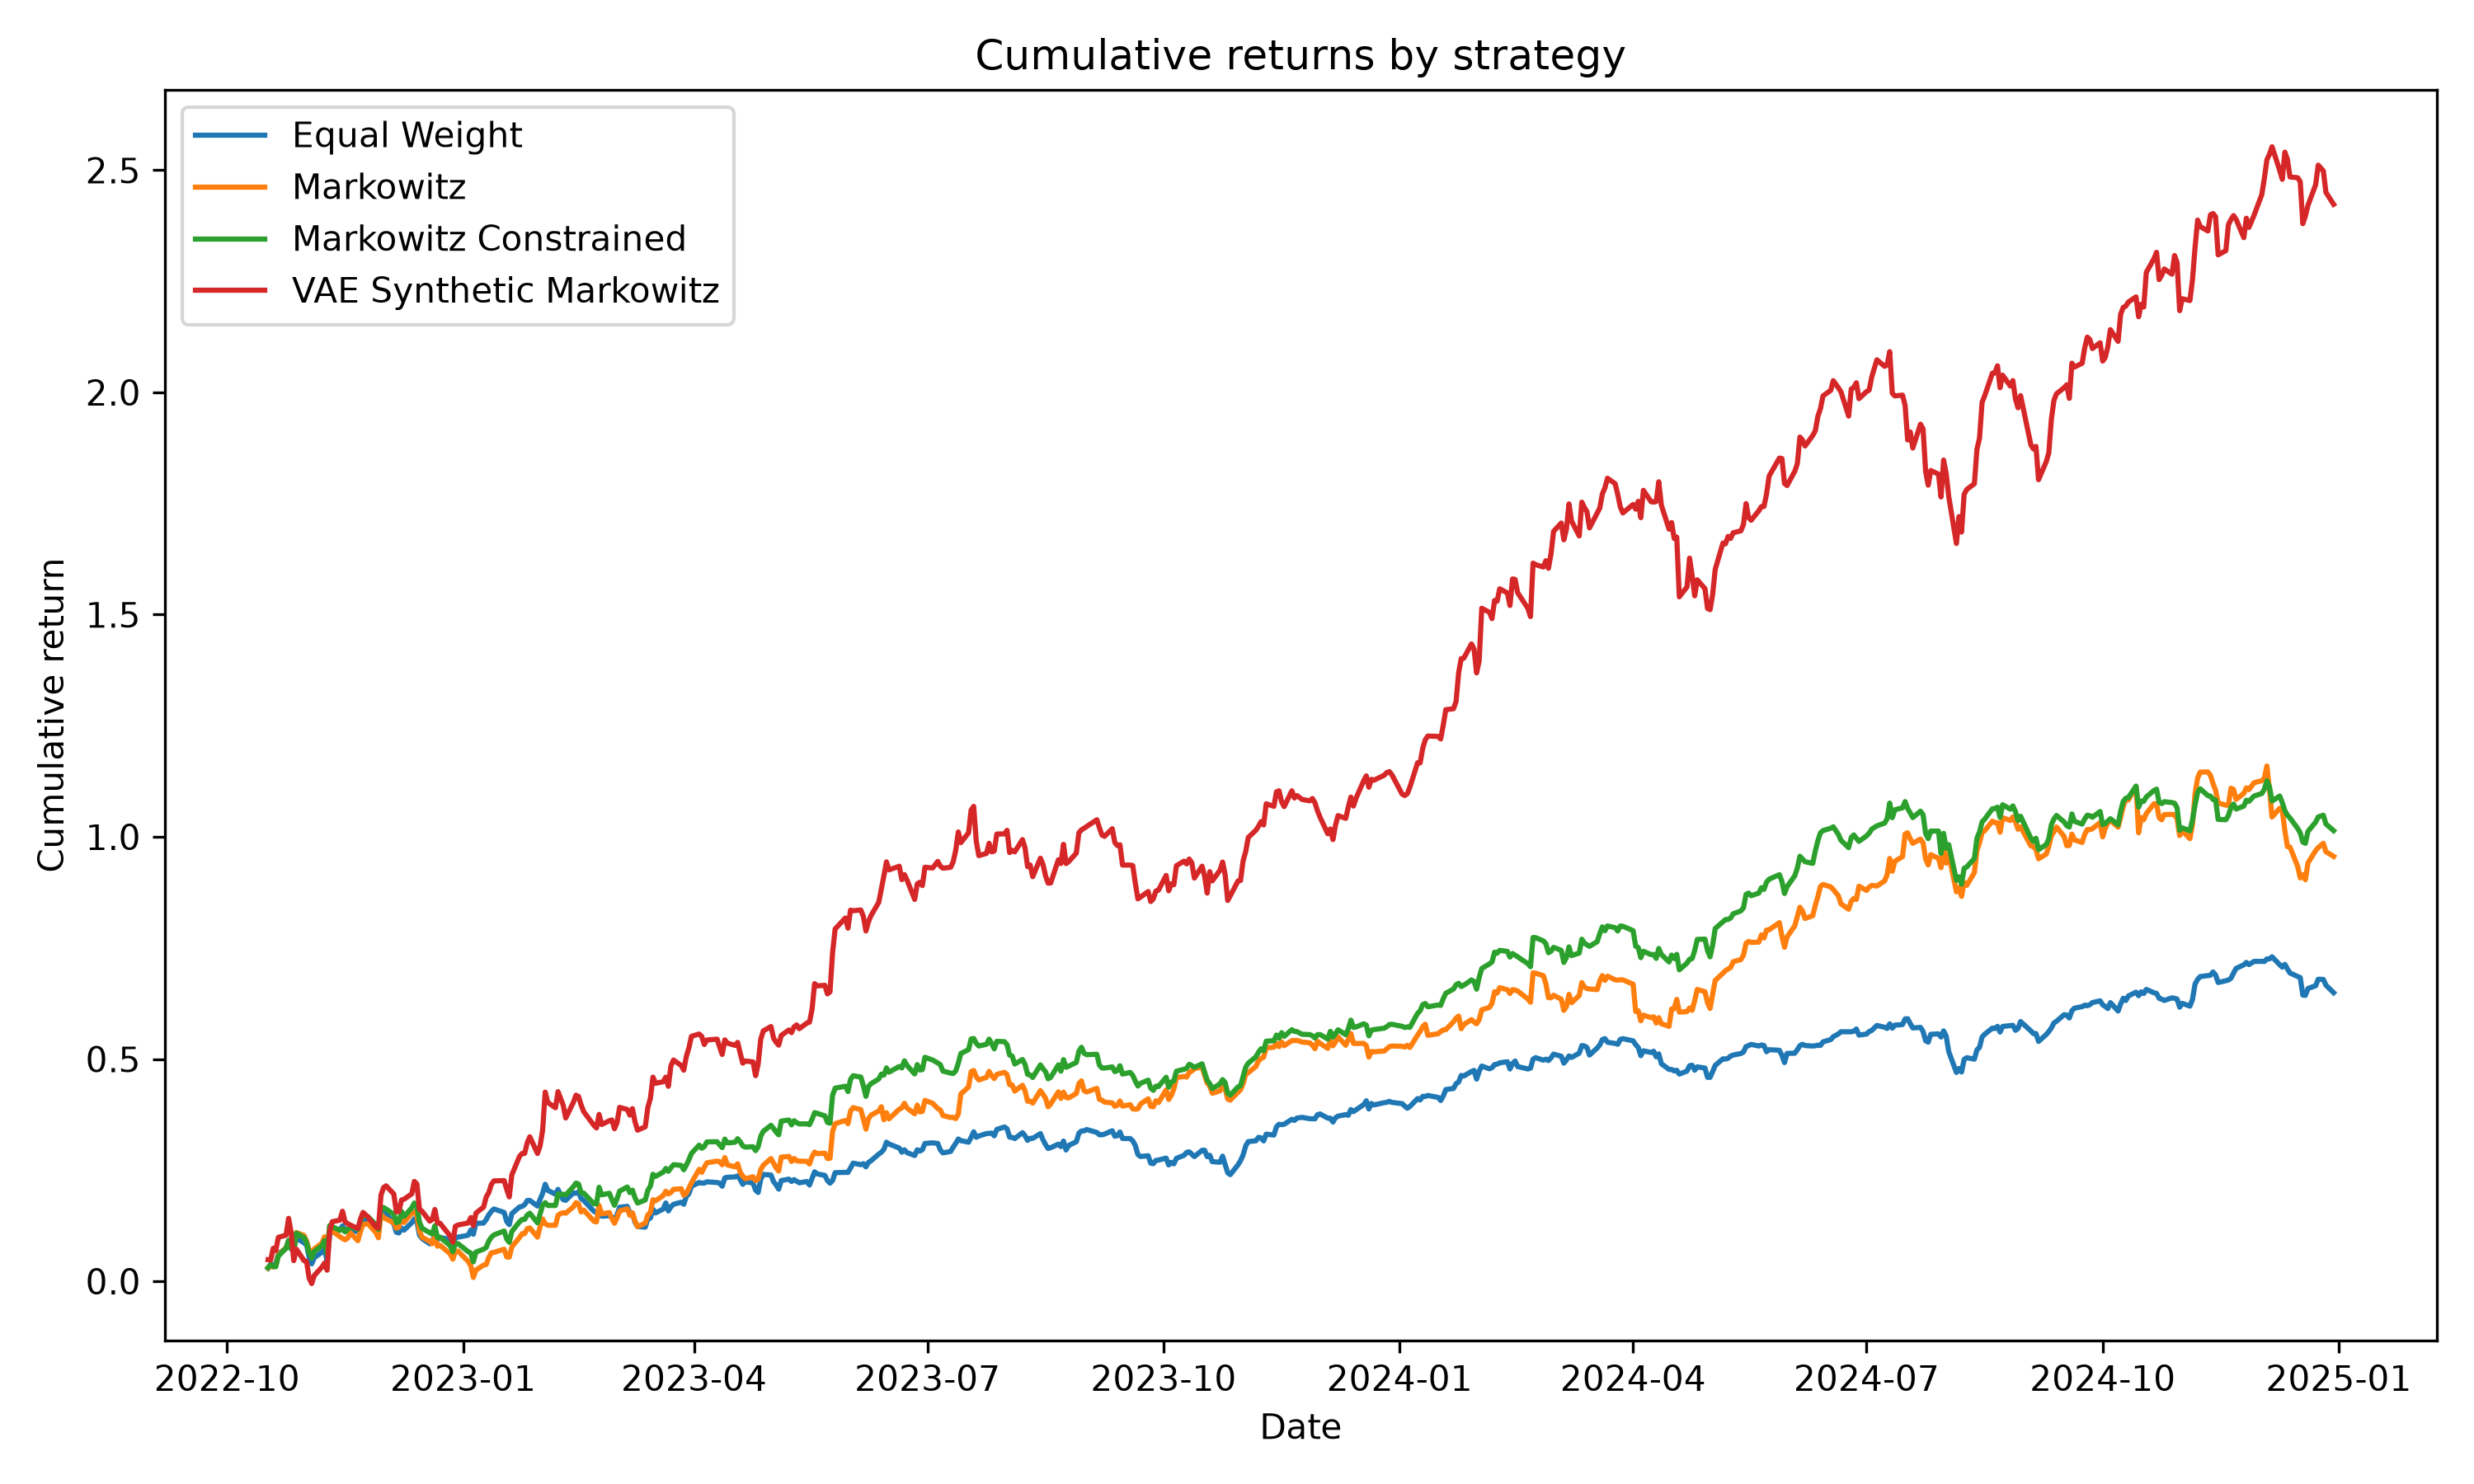
\includegraphics[width=0.9\textwidth]{../figures/strategy_cumulative_returns.png}
\caption{Evolución acumulada de las estrategias durante el periodo de test. Fuente: elaboración propia a partir de los retornos generados por el pipeline.}
\label{fig:resultados_acumulados}
\end{figure}

\subsection{Lectura por estrategia}

La equiponderada es el resultado más conservador de la tabla. Obtiene el menor retorno, pero también la menor volatilidad y el \textit{drawdown} menos profundo. Su Sharpe de 1,88 queda muy próximo al 1,89 de Markowitz clásico. Esto recuerda que una regla simple puede ser competitiva cuando la incertidumbre de estimación es elevada.

Markowitz clásico eleva el retorno anualizado hasta 35,69~\%, pero su volatilidad sube a 18,86~\% y la caída máxima a -12,78~\%. La mejora casi nula de Sharpe respecto a equiponderación indica que el retorno adicional viene acompañado de riesgo proporcional. La concentración observada en sus pesos es coherente con la conocida sensibilidad de las soluciones media-varianza.

La restricción del 20~\% produce un compromiso más favorable en este test: aumenta el retorno frente a Markowitz, reduce volatilidad y \textit{drawdown}, y eleva Sharpe a 2,20. Este resultado no implica que el límite del 20~\% sea óptimo, pero muestra que una restricción interpretable puede actuar como regularización de la cartera.

La estrategia VAE alcanza los mayores retorno y Sharpe. Simultáneamente presenta la mayor volatilidad y la caída más profunda. Su perfil es, por tanto, más agresivo. La diferencia no puede atribuirse simplemente a «inteligencia artificial»: surge de medias y covarianzas estimadas sobre escenarios que asignan pesos distintos y pueden favorecer activos con buen comportamiento posterior.

\subsection{Por qué el resultado VAE puede ser elevado}

Existen varias explicaciones compatibles. En primer lugar, el test cubre un periodo concreto y algunos activos seleccionados experimentaron fuertes revalorizaciones. Una cartera concentrada en ellos amplifica el retorno. En segundo lugar, el VAE suaviza volatilidades en parte de sus muestras, como muestra \texttt{vae\_synthetic\_summary.csv}; una covarianza sintética reducida puede hacer atractivos ciertos pesos. En tercer lugar, pequeños errores en medias diarias se amplifican al anualizar y optimizar Sharpe.

También existe selección experimental: la memoria presenta una configuración principal, no una distribución de resultados sobre numerosas semillas y ventanas. Aunque el test no se usó para entrenar el VAE ni calcular pesos, haber analizado el mismo periodo durante el desarrollo puede generar decisiones indirectamente adaptadas a él. La comparación multimodelo mejora la transparencia, pero no reemplaza una validación anidada.

\subsection{Relación con la calidad generativa}

La cartera VAE obtiene buen Sharpe aun cuando la comparación de modelos detecta errores apreciables de volatilidad y correlación sintéticas. No hay contradicción matemática: la utilidad para una cartera depende de cómo esas diferencias alteren el óptimo y del comportamiento posterior de los activos. Sin embargo, sí existe una advertencia: un buen resultado financiero en un único test no prueba que la distribución generada sea fiel.

Por esta razón se mantienen separados tres planos: reconstrucción, similitud estadística y rendimiento. El VAE base logra el menor error de medias sintéticas entre los tres modelos comparados, pero el AE reproduce mejor volatilidades y correlaciones con el procedimiento ensayado. Una ampliación debería construir carteras desde ambos y repetir el proceso en múltiples ventanas.

\subsection{Evaluación comparativa y validez}

Bajo el periodo analizado, los resultados sugieren que modificar la estimación de parámetros mediante escenarios puede producir asignaciones con mejores métricas de rentabilidad y Sharpe. También confirman el valor práctico de restricciones de concentración. La estrategia VAE fue superior en este experimento concreto, pero un único universo de activos y un único corte temporal no bastan para afirmar superioridad general frente a Markowitz o equiponderación, ni para sostener que el modelo prediga el mercado.

No se modelan comisiones, horquillas, impuestos ni impacto de mercado. Tampoco hay rebalanceo, por lo que no se evalúa rotación. El tipo libre de riesgo se fija en cero y las métricas no incluyen VaR o CVaR. Finalmente, un solo test carece de la diversidad de una validación \textit{walk-forward}. Estas condiciones hacen que la tabla deba interpretarse como resultado académico reproducible, no como expectativa de inversión.

\subsection{Síntesis de resultados}

El resultado de la cartera VAE no debe interpretarse como una predicción de rentabilidad futura, sino como una evidencia experimental de que la estimación de parámetros mediante escenarios sintéticos puede alterar de forma sustancial la solución óptima bajo el periodo analizado.

La equiponderación minimiza riesgo observado; Markowitz aumenta retorno sin mejorar apenas Sharpe; la restricción del 20~\% mejora el equilibrio; y la estimación VAE produce el mayor retorno y Sharpe con mayor riesgo. El hallazgo central no es una garantía de rentabilidad, sino que la fuente de escenarios altera materialmente los parámetros, los pesos y el resultado fuera de muestra. Esa sensibilidad justifica profundizar en validación temporal, estabilidad y calidad de colas antes de cualquier uso práctico.
